\documentclass[12pt, notitlepage, final]{article} 

\newcommand{\name}{Vince Coghlan}

%\usepackage[dvips]{graphics,color}
\usepackage{amsfonts}
\usepackage{amssymb}
\usepackage{amsmath}
\usepackage{latexsym}
\usepackage{enumerate}
\usepackage{amsthm}
%\usepackage{nccmath}
\usepackage{setspace}
\usepackage[pdftex]{graphicx}
\usepackage{epstopdf}
%\usepackage[siunitx]{circuitikz}
\usepackage{tikz}
\usepackage{float}
%\usepackage{cancel} 
\usepackage{setspace}
%\usepackage{overpic}
\usepackage{mathtools}
\usepackage{listings}
\usepackage{color}
%\usepackage{gensymb}

\usetikzlibrary{calc}
\usetikzlibrary{matrix}
\usetikzlibrary{positioning}

\numberwithin{equation}{section}
\DeclareRobustCommand{\beginProtected}[1]{\begin{#1}}
\DeclareRobustCommand{\endProtected}[1]{\end{#1}}
\newcommand{\dbr}[1]{d_{\mbox{#1BR}}}
\newtheorem{lemma}{Lemma}
\newtheorem*{corollary}{Corollary}
\newtheorem{theorem}{Theorem}
\newtheorem{proposition}{Proposition}
\theoremstyle{definition}
\newtheorem{define}{Definition}
\newcommand{\column}[2]{
\left( \begin{array}{ccc}
#1 \\
#2
\end{array} \right)}

\newdimen\digitwidth
\settowidth\digitwidth{0}
\def~{\hspace{\digitwidth}}

\setlength{\parskip}{1pc}
\setlength{\parindent}{0pt}
\setlength{\topmargin}{-3pc}
\setlength{\textheight}{9.0in}
\setlength{\oddsidemargin}{0pc}
\setlength{\evensidemargin}{0pc}
\setlength{\textwidth}{6.5in}
\newcommand{\answer}[1]{\newpage\noindent\framebox{\vbox{{\bf ECEN 5018 Spring 2014} 
\hfill {\bf \name} \vspace{-1cm}
\begin{center}{Homework \#1}\end{center} } }\bigskip }

\DeclareMathOperator*{\argmin}{arg\,min}

%absolute value code
\DeclarePairedDelimiter\abs{\lvert}{\rvert}%
\DeclarePairedDelimiter\norm{\lVert}{\rVert}
\makeatletter
\let\oldabs\abs
\def\abs{\@ifstar{\oldabs}{\oldabs*}}
%
\let\oldnorm\norm
\def\norm{\@ifstar{\oldnorm}{\oldnorm*}}
\makeatother

\def\dbar{{\mathchar'26\mkern-12mu d}}
\def \Frac{\displaystyle\frac}
\def \Sum{\displaystyle\sum}
\def \Int{\displaystyle\int}
\def \Prod{\displaystyle\prod}
%\def \P[x]{\Frac{\partial}{\partial x}}
%\def \D[x]{\Frac{d}{dx}}
\newcommand{\PD}[2]{\frac{\partial#1}{\partial#2}}
\newcommand{\PF}[1]{\frac{\partial}{\partial#1}}
\newcommand{\DD}[2]{\frac{d#1}{d#2}}
\newcommand{\DF}[1]{\frac{d}{d#1}}
\newcommand{\fix}[2]{\left(#1\right)_#2}
\newcommand{\ket}[1]{|#1\rangle}
\newcommand{\bra}[1]{\langle#1|}
\newcommand{\braket}[2]{\langle #1 | #2 \rangle}
\newcommand{\bopk}[3]{\langle #1 | #2 | #3 \rangle}
\newcommand{\Choose}[2]{\displaystyle {#1 \choose #2}}
\newcommand{\proj}[1]{\ket{#1}\bra{#1}}
\def\del{\vec{\nabla}}
\newcommand{\avg}[1]{\langle#1\rangle}
\newcommand{\piecewise}[4]{\left\{\beginProtected{array}{rl}#1&:#2\\#3&:#4\endProtected{array}\right.}
\newcommand{\systeme}[2]{\left\{\beginProtected{array}{rl}#1\\#2\endProtected{array}\right.}
\def \KE{K\!E}
\def\Godel{G$\ddot{\mbox{o}}$del}

\onehalfspacing

\begin{document}

\answer{}

1) \textbf{Tragedy of the Commons:} Suppose 10 families share a plot of land. A goat that grazes on fraction $a \in [0,1]$ of land produces
\[
b = e^{1-\frac{1}{10a}}
\]
bucket of milk. A social planner would like to maximize total milk production. How many goats should be owned among the families to maximize total milk production? Now consider the situation where each family gets to keep only their own milk. Model this situation as a strategic game and identify all Nash equilibria. How does the total milk production change as we transition from a social optimization to a family optimization? Assume throughout that land is divided equally amongst the goats.

In the case where the production of milk is communal, we can find the optimal goat population quite easily.  One goat would provide $e^{\frac{9}{10}} \approx 2.46$ buckets of milk. Two would provide $2\cdot e^{\frac{4}{5}} \approx 4.45$.  We can find the maximum of a total milk function $M = x\cdot e^{1 - \frac{1}{10/x}}$ to be $10$ goats, when they would produce exactly 10 buckets of milk, or 1 bucket per family.  Obviously no family wants no milk, so initially each family will want at least one goat.  This situation shows that for any one family $i$, goat distribution profile $g$, and a milk per family production of $b_i$, then adding a goat would change $b_i$ like so:
\[
b_i(g^*_i, g^*_{-i}) = \frac{1}{a}\cdot e^{1-\frac{1}{10a}} \text{, } b_i(g_i, g^*_{-i}) = \frac{2}{a-1} \cdot e^{1 - \frac{1}{10(a-1)}}
\]
Note that it matters not the goat distribution of the other families, this will always be the case.  These values can be visualized:
\begin{figure}[H]
\begin{center}
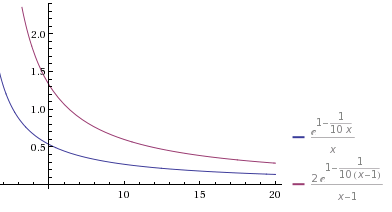
\includegraphics[width=10cm]{f1}
\end{center}
\end{figure}
It can be shown that one goat is better than none, and an extra goat will provide more milk, and thus:
\[
b_i(g^*_i, g^*_{-i}) < b_i(g_i, g^*_{-i})
\]
Meaning that there are no Nash equilibria.  This means that everyone will have as many goats as they can fit on the land.  In our idealized mathy context, and infinite amount of goats, and zero milk for anybody, since $b_i(g) = e^{-\infty} = 0$.\\
\\

2) \textbf{Routing}: Consider the routing problem discussed in lecture. In this routing problem, there is 1 unit of divisible traffic that needs to be routed from the start to the destination.  There are two possible routing choices either the \textbf{High} road or the \textbf{Low} road. The cost on the high road is $c_H(x) = x$ where $x$ is the fraction of traffic using the high road. The cost on the low road is $c_L(x) = 1$ for all $x \in [0, 1]$.
\begin{enumerate}[(a)]
\item If a social planner controls all traffic, what is the routing profile that minimizes the total cost? The total cost of a routing profile $(f_H, f_L)$ is $f_Hc_H(f_H)+f_Lc_L(f_L)$ where $f_L$, $f_H$ are the fractions of traffic on the high and low road.
\item Suppose there are two decision makers that each control $1/2$ of the traffic. Each decision maker only cares about the total cost of his traffic. Model this situation as a strategic game and analyze the Nash equilibria. How does the total cost compare with the total cost from part (a).
\item Suppose there are $n$ decision makers that each control $1/n$ of the traffic. Model this situation as a strategic game and analyze the Nash equilibria. How does the total cost compare with the total cost from part (a). What happens as $n \to \infty$?
\end{enumerate}

(a) A social planner wants to minimize the total congestion in the system.  A simple equation for the total cost can be made: $C = f_Hc_H(f_H) + f_Lc_L(f_L) = (f_H)^2 + f_L$  We know that the fraction on the low road is $1 - f_H$. and thus $C = (f_H)^2 + 1 - f_H$ which is minimized when the derivative is zero.  $2f_H-1=0$, $f_H = \frac{1}{2}$, and thus $f_L = \frac{1}{2}$.

(b) Now we have two decision makers.  We can imagine initially if both planner's have their traffic split among the two roads that they would want to change that.  Each player realizes that they can move traffic to the high road and decrease costs.  The cost for either agent can be seen below:
\[
u_i(f^H_1,f^H_2) = f^H_i(f^H_1+f^H_2)+(0.5-f^H_i)
\]
This allows us to compute the best response of player 1:
\[
b_1(x) = \underset{0\le f^H_1\le 0.5}\argmin f^H_1 \cdot (x + f^H_1) + (0.5 - f^H_1)
\]
The derivative set to 0 will find us the equilibrium.
\[
x + 2\cdot f^H_1 - 1 = 0 \Rightarrow b_1(x) = \frac{1}{2} - \frac{x}{2} \Rightarrow b_2(y) = \frac{1}{2} - \frac{y}{2}
\]
These best responses can be seen graphically:
\begin{figure}[H]
\begin{center}
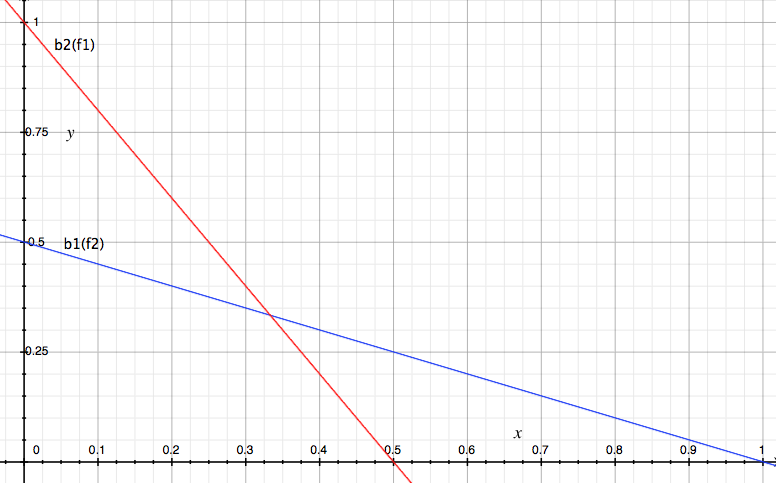
\includegraphics[width=14cm]{f2}
\end{center}
\end{figure}

There will occur a Nash Equilibrium when these two function are equalized.
\[
f^H_1=b_1(f^H_2)\text{, }f^H_2=b_2(f^H_1) \Rightarrow f^H_i = \frac{1}{3}
\]

(c) If there are $n$ players then the costs will look like the following:
\[
u_i(f^H_i, f^H_{-i}) = f^H_i(f^H_1 + f^H_2 + ... + f^H_n) + (\frac{1}{n} - f^H_i)
\]
\[
b_i(x) = \underset{0\le f^H_i \le \frac{1}{n}}\argmin (f^H_i)^2 + f^H_i \cdot f^H_{-i} + \frac{1}{n} - f^H_i
\]
In a similar way:
\[
2\cdot f^H_i + (n-1)\cdot x - 1 = 0 \Rightarrow b_i(x) = \frac{1}{2} - \frac{(n-1)\cdot x}{2}
\]
We can see how this plays out for various values of n (note that I'm only plotting two of the agents, I simply don't have enough dimensions to plot any more):
\begin{figure}[H]
\begin{center}
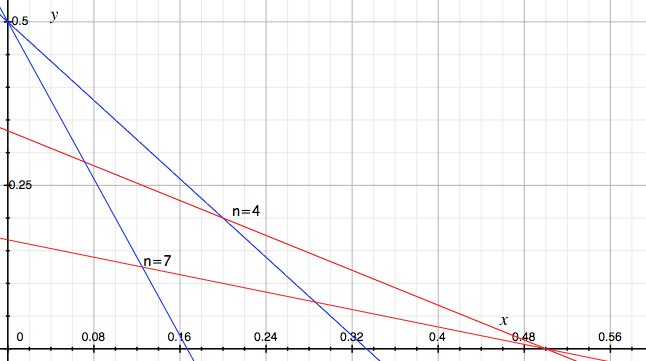
\includegraphics[width=14cm]{f3}
\end{center}
\end{figure}
It is clear from the best response equation and the graph that as $n\to \infty$ the best response off all users will be to send all the users on the high road.\\

3) \textbf{18.2:} Formulate a first price auction as a strategic game and analyze its Nash equilibria.  In particular, show that in all equilibria player 1 obtains the object.

In this strategic game each player $i$ will have some valuation for the item: $v_1 > v_2 > ... > v_n$ and each player will make a bid $b_1, b_2, ..., b_n$.  The winner in the game is the player with the highest bid, he will pay his bid.  The payoff matrix for any player $i$ will be as follows:
\[
\text{If } b_i > \max\{b_{-i}\}: v_i - b_i
\]
\[
\text{If } b_i < \max\{b_{-i}\}: 0
\]
Since no player has an incentive to bid higher than their value, player one is going to bid slightly higher than the next highest bid, in order to attain the object.  He wins, and ends up with a payoff of $v_i - \max\{b_{-i}\}$ which is a positive number.  This is a Nash equilibrium since player 1 would not want to lose that payoff, and every other player would not want to bid more than their valuation.\\

4) \textbf{18.3:} Show that in a second price auction the bid $v_i$ of any player $i$ is a weakly dominant action: player $i$'s payoff when he bids $v_i$ is at least as high as his payoff when he submits any other bid, regardless of the actions of the other players.  Show that nevertheless there are ("inefficient") equilibria in which the winner is not player 1.

for player $i$'s payoff when he bids his value to be at least as high as when another bid is made, regardless of other player's actions, we would need to iterate through every possible situation and check the math.
\[
\text{Let }\bar{b}=max\{b_{-i}\}
\]
\[
\text{If } v_i = b_i \Rightarrow u_i(b_i=v_i, b_{-i}) = v_i - \bar{b} \text{ (note number $>$ 0)}
\]
\[
\text{If } b_i>v_i
\]
\[
\bar{b} < v_i < b_i \Rightarrow u_i(b_i, b_{-i}) = v_i - \bar{b}
\]
\[
v_i < \bar{b} < b_i \Rightarrow u_i(b_i, b_{-i}) = v_i - \bar{b}
\]
\[
v_i < b_i < \bar{b} \Rightarrow u_i(b_i, b_{-i}) = 0
\]
\[
\text{If } b_i<v_i
\]
\[
\bar{b} < b_i < v_i \Rightarrow u_i(b_i, b_{-i}) = v_i - \bar{b}
\]
\[
b_i < \bar{b} < v_i \Rightarrow u_i(b_i,  b_{-i}) = 0
\]
\[
b_i < v_i < \bar{b} \Rightarrow u_i(b_i, b_{-i}) = 0
\]
In this situation the inefficient equilibria would be the situations in which player 1 loses, even though he values the item the most.  These are the third, the fifth, and the sixth of the above situations.

5) \textbf{18.5:} (A war of attrition)  Two players are involved in a dispute over an object.  The value of the object to player $i$ is $v_i > 0$.  Time is modeled as a continuous variable that starts at 0 and runs indefinitely.  Each player chooses when to concede the object to the other player; if the first player to concede does so at time $t$, the other player obtains the object at that time.  If both players concede simultaneously, the object is split equally between them, player $i$ receiving a  payoff of $v_i/2$. Time is valuable: until the first concession each player loses one unit of payoff per unit of time.  Formulate this situation as a strategic game and show that in all Nash equilibria one of the players concedes immediately. 

A player's strategy $a_i$ is the time at which they concede.  The player with the largest of this value wins.  The payoff for winning is $v_i - \min(a_i)$, the other player loses $\min(a_i)$.  If the times are the same then both players win $v_i/2 - a_i$.   We know that they cannot concede at different times after $t=0$, because if they did, then one of the players would be playing a strategy that would be less valuable then conceding immediately.  If the times to concede are equal, then one player would rather wait a very small amount of time to get the extra value.  So there is no Nash equilibrium when one player does not concede immediately.  The only Nash equilibria are when player 1 concedes, or player 2 concedes at $t=0$.

6) \textbf{19.1:} (A location game) Each of $n$ people chooses whether or not to become a political candidate, and if so which position to take.  There is a continuum of citizens, each of whom has a favorite position; the distribution of favorite positions is given by a density function $f$ on [0,1] with $f(x) > 0$ for all $x \in [0,1]$.  A candidate attracts the votes of those citizens whose favorite positions are closer to his position than to the position of any other candidate; if k candidates choose the same position then each receives the fraction $1/k$ of the votes that the position attracts.  The winner of the competition is the candidate who receives the most votes.  Each person prefers to be the unique winning candidate than to tie for first place, prefers to tie for first place than to stay out of the competition, and prefers to stay out of the competition than to enter and lose. Formulate this situation as a strategic game, find the set of Nash equilibria when $n=2$, and show that there is no Nash equilibrium when $n=3$.

For the first case, when $n = 2$, there is a Nash equilibrium when $x_1 = x_2 = 1/2$.  This is because that no matter what one player can do, the other can always wither beat or tie him.  if they both pick $1/2$ then its a tie, and that is the best either can do.  If one player picks a different $x$ then they can be beat by the other playing $1/2$.  For the case where $n=3$ there are no Nash equilibria.  Never would three people concede, because one could easily win.  Never would one or two people concede because one could increase to a tie by playing.  This means all we have left is all of them are playing.  In this case, they can't all tie, because if one moves his $x$ just a little to the right or left, he could get way more votes.  This means that there are no Nash equilibria in this game, because every candidate could do better.



















\end{document}